\section{Further empirical results}

\subsection{UCI datasets}
\label{sec:uci-experiments}

We revisit the experiments in Section~\ref{sec:motivation-exp}, focusing on
evaluating our methodology for robust predictive inference.  Our goal here
is to show that when our estimate of the amount of shift is comparable to
the actual amount of shift, our methodology delivers coverage without
inflating prediction sets too much.  Accordingly, throughout these
experiments, we fix the desired robustness level $\rho = .01$, corresponding
(approximately) to the median chi-squared divergence between the natural and
tilted empirical distributions across the nine data sets and values of the
tilting parameter $a$.  We therefore expect
Algorithm~\ref{alg:rho-selection-procedure}, which emphasizes robustness to
worst-case shifts, to restore the coverage level for the tiltings from
Section~\ref{sec:motivation-exp} that possess (roughly) this level of shift.

Figure \ref{fig:cvgs_only_chisq} presents the results for the chi-squared
divergence (the results for the Kullback-Leibler divergence are similar).
Although not perfect, we see that the methodology often restores validity
for the shifts from Section~\ref{sec:motivation-exp}.  We see clearly
improved performance over the standard conformal methodology on the abalone,
delta ailerons, kinematics, puma, and airfoil datasets (compare to
Figure~\ref{fig:cvgs_only_std}).  On all of these datasets, the robust
methodology consistently yields average coverage above the nominal level,
while standard conformal fails to cover on each of the datasets.  Treating
the test sample as truth, we evaluate the median chi-squared divergence
between these natural and shifted distributions across values of the tilting
parameter $a$; the divergence values are .03, .02, .04, .05, and 3.65,
respectively, while the level of divergence for the remaining datasets
(ailerons---which still covers---banking, and Boston and California housing)
is roughly twice as large, which explains the loss in coverage.  We note in
passing that in other experiments we omit for brevity, the trends above hold
for other types of shifts.

\begin{figure}[h!]
    \centering
    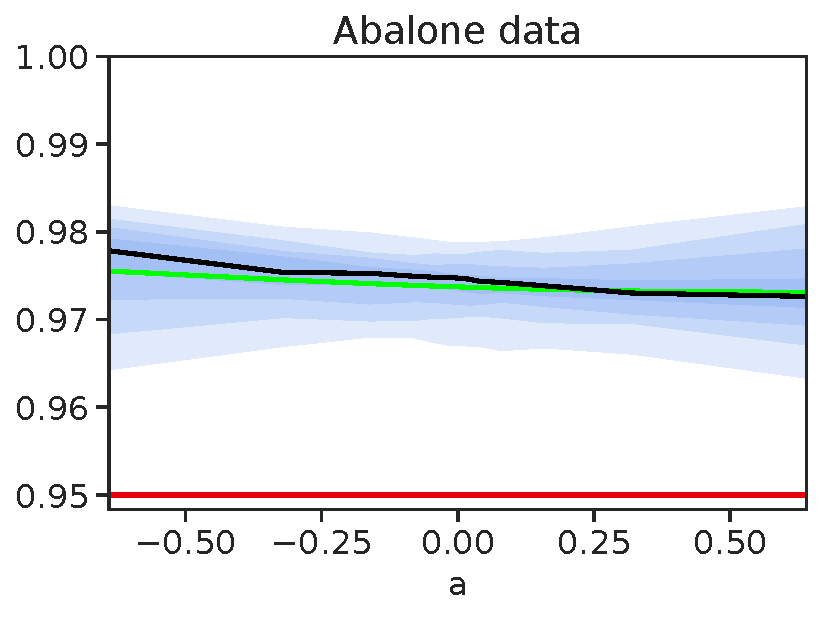
\includegraphics[width=0.3\linewidth]{uci/abalone_coverage_Chi-squared_I-B.pdf}
    \hfill
    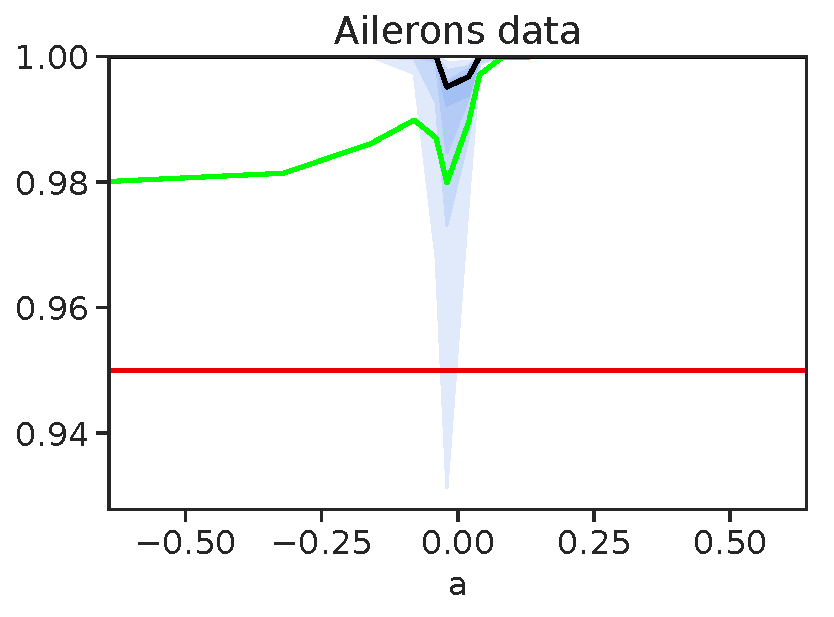
\includegraphics[width=0.3\linewidth]{uci/ailerons_coverage_Chi-squared_I-B.pdf}
    \hfill
    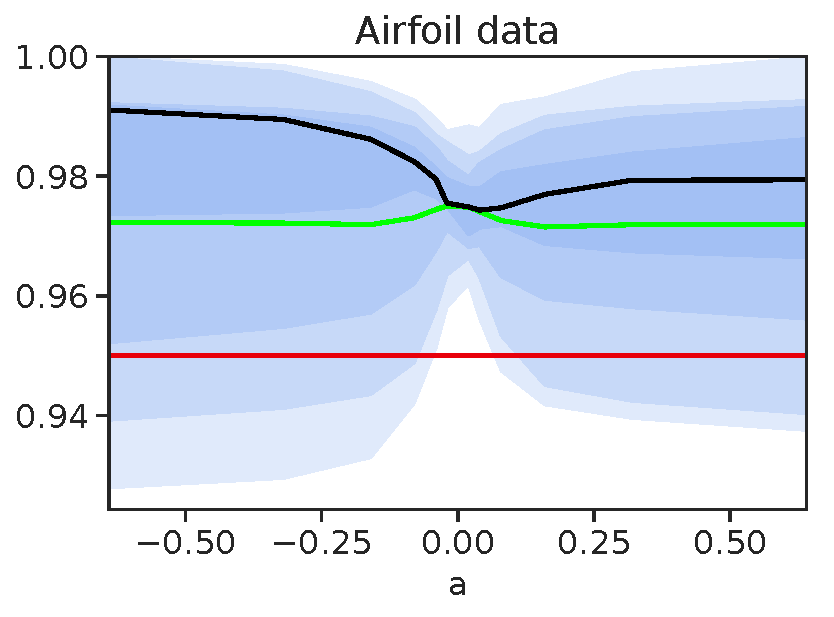
\includegraphics[width=0.3\linewidth]{uci/airfoil_coverage_Chi-squared_I-B.pdf}
    \\
    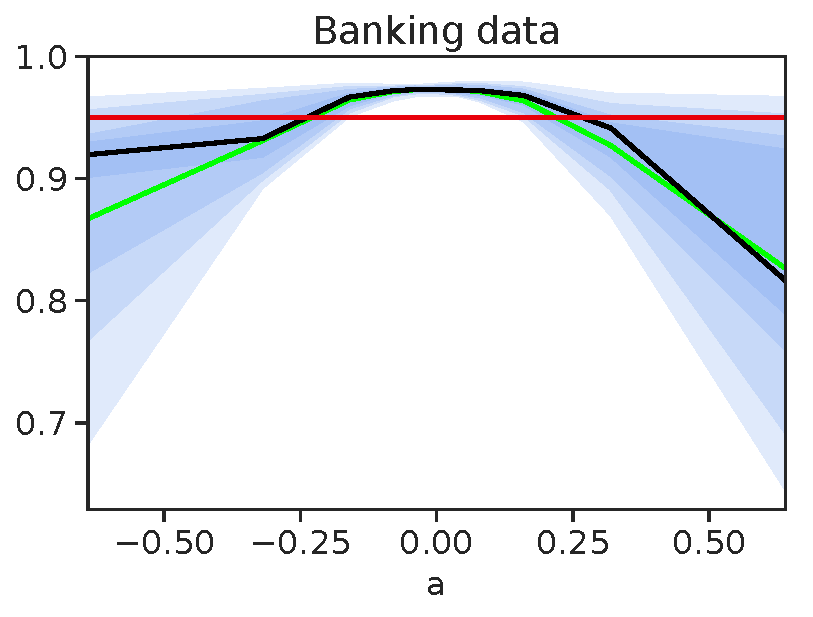
\includegraphics[width=0.3\linewidth]{uci/bank_coverage_Chi-squared_I-B.pdf}
    \hfill
    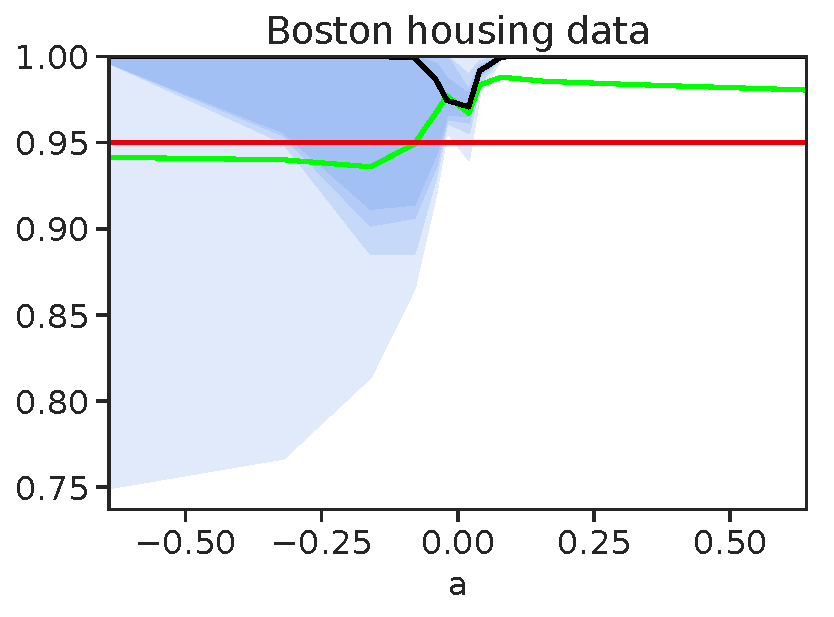
\includegraphics[width=0.3\linewidth]{uci/bos_coverage_Chi-squared_I-B.pdf}
    \hfill
    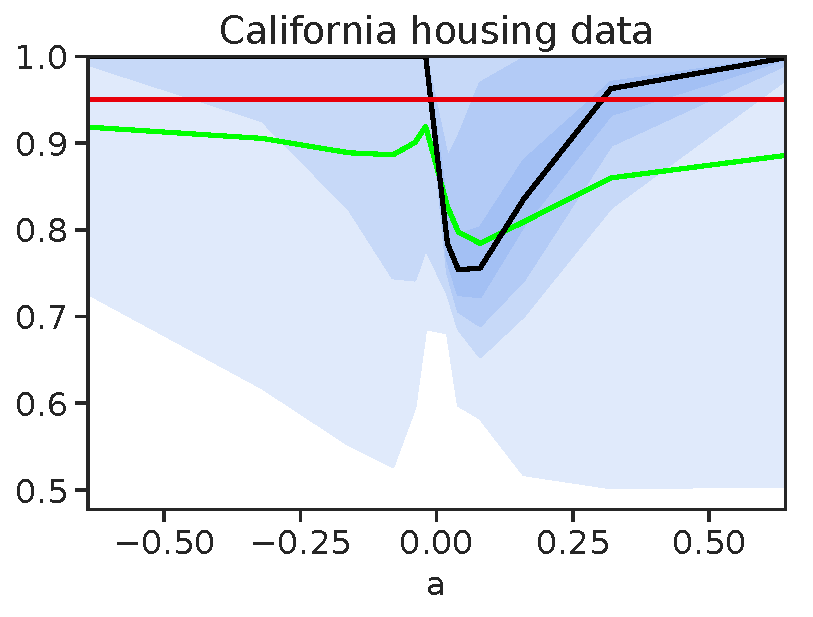
\includegraphics[width=0.3\linewidth]{uci/ca_coverage_Chi-squared_I-B.pdf}
    \\
    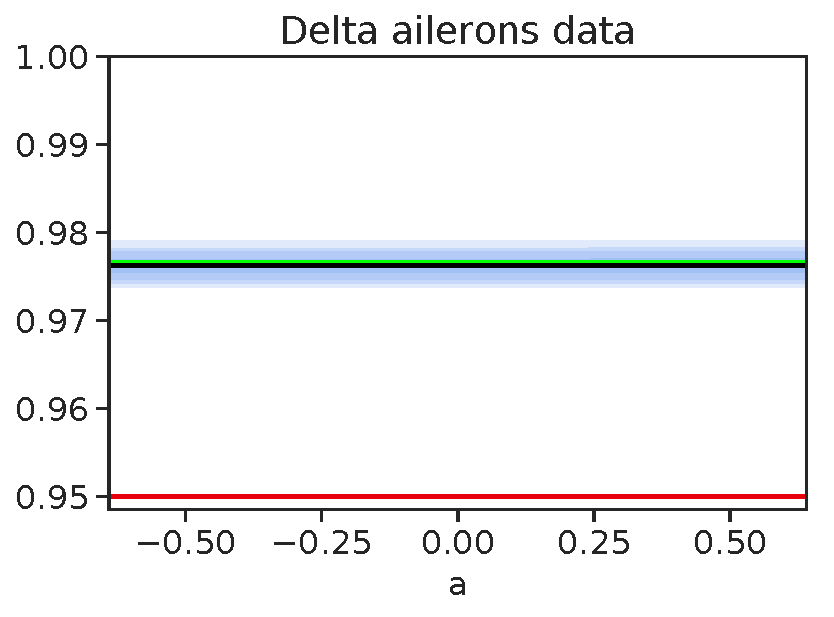
\includegraphics[width=0.3\linewidth]{uci/delta_coverage_Chi-squared_I-B.pdf}
    \hfill
    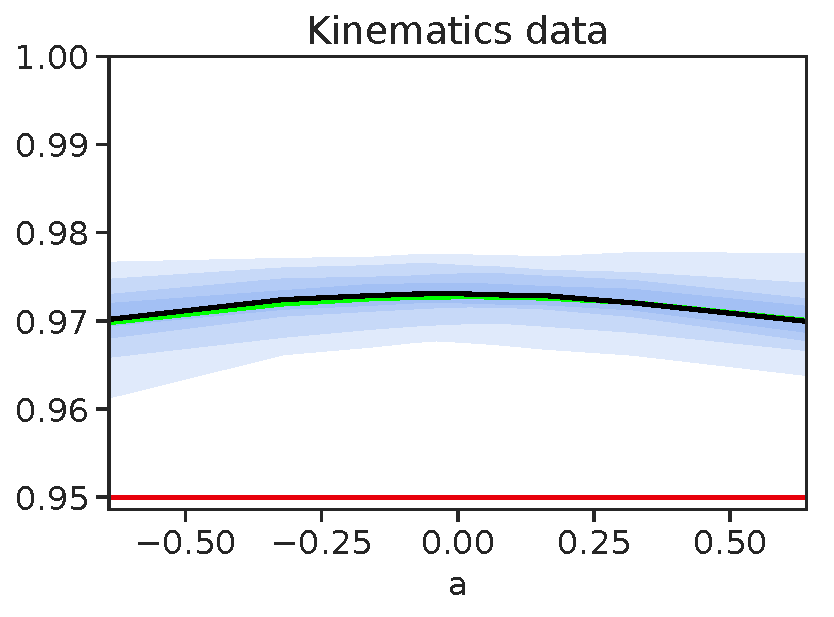
\includegraphics[width=0.3\linewidth]{uci/kin_coverage_Chi-squared_I-B.pdf}
    \hfill
    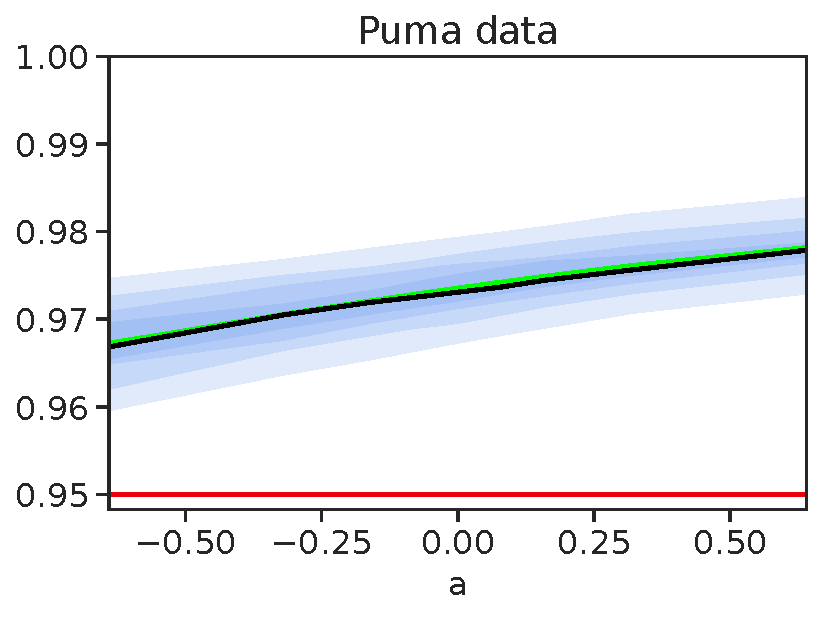
\includegraphics[width=0.3\linewidth]{uci/puma_coverage_Chi-squared_I-B.pdf}  
    \caption{Empirical coverage for the prediction sets generated by the
    chi-squared divergence, following the same experimental setup from Section
    \ref{sec:motivation-exp}. The horizontal axis gives the value of the tilting
    parameter $a$; the vertical the coverage level. A green line marks the
    average coverage, a black line marks the median coverage, and the horizontal
    red line marks the nominal coverage $.95$. The blue bands show the coverage
    at various deciles.}
    \label{fig:cvgs_only_chisq}
\end{figure}

\subsection{COVID-19 forecasting}
\label{sec:real-experiments-covid}

Our final evaluation of prediction accuracy under shifts is to predict test
positivity rates for COVID-19, in each of $L = 3{,}140$ United States
counties in a time series over $T = 34$ weeks from January through the
beginning of August 2021, using demographic features.  As a
non-stationary time series, robustness is essential here as a fixed model of
course cannot adapt to the underlying distributional changes.

Our prediction task is as follows.  For each of $t=1,\ldots,T$ weeks, and at
each of $\ell=1,\ldots,L$ locations (counties), we observe a
real-valued response $Y_{\ell, t} \in [0,1]$, $\ell=1,\ldots,L$,
$t=1,\ldots,T$, measuring the fraction of people with COVID-19.
We use data from the DELPHI group at Carnegie Mellon University
\citep{ArnoldBiBrCoFaGrMaReTi21,Tibshirani20} and consider a similar
featurization, using the following
trailing average features within each county: (1)
the number of COVID-19 cases per 100{,}000 people; (2) the number of doctor
visits for COVID-like symptoms; and (3) the number of responses
to a Facebook survey indicating respondents have COVID-like symptoms.  We
standardize both the features and responses so that they lie in $[0,1$], and
collect the features into vectors $X_{\ell, t} \in \R^3$, $\ell=1,\ldots,L$,
$t=1,\ldots,T$.

At each week $t = 1, 4, 7, \ldots$, 
we fit a simple logistic model where for a fixed $t$, we compute
\begin{equation}
  \label{eqn:logistic-goof}
  (\hat \alpha^{(t)}, \hat \beta^{(t)}) \in
  \argmin_{\alpha \in \R, \beta \in \R^d}
  ~
  \sum_{\ell = 1}^L
  \left[\log(1 + e^{\alpha + X_{\ell,t}^T \beta}) -
    Y_{\ell,t+1} (\alpha + X_{\ell,t}^T \beta)\right]
  %% \underset{\alpha \in \R, \beta \in \R^d}{\argmin} & \sum_{\ell=1}^L \big| Y_{\ell,t+1} - ( \alpha + X_{\ell,t}^T \beta ) \big|.
  %%   \end{array}
\end{equation}
We treat the data at the weeks $t=2,5,8,\ldots$ as the validation set, the
data at the remaining weeks $t=3,6,9,\ldots$ as the test set, so that at
each time $t$ we fit the single most recent time period's data. We make
predictions on a new example $x$ at time $t$ via the logistic link
\begin{equation*}
  \what{y} = \frac{e^{\hat{\alpha}^{(t)} + x^T \hat{\beta}^{(t)}}}{1 +
    e^{\hat{\alpha}^{(t)} + x^T \hat{\beta}^{(t)}}}.
\end{equation*}


%% At each week $t=1,4,7,\ldots$, we fit a simple logistic model via least absolute deviations regression, i.e., for a fixed $t$, we compute
%% % (including the global model used on the first pass that we mentioned earlier) 
%% \begin{equation} \label{eq:LAD}
%%     \begin{array}{ll}
%%         (\hat \alpha^{(t)}, \hat \beta^{(t)}) \in \underset{\alpha \in \R, \beta \in \R^d}{\argmin} & \sum_{\ell=1}^L \big| Y_{\ell,t+1} - ( \alpha + X_{\ell,t}^T \beta ) \big|.
%%     \end{array}
%% \end{equation}
%% Letting $\hat \mu^{(t)}(X_{\ell, t+1}) = \hat \alpha^{(t)} + X_{\ell, t+1}^T \hat \beta^{(t)}$ and
%% \[
%%     g(z) = \log \Big( \frac{z+c}{1-z+c} \Big)
%% \]
%% denote the logit link function, the simple logistic model makes a prediction at $X_{\ell, t+1}$ by forming
%% \begin{equation*}
%%     g^{-1} \big( \hat \mu^{(t)}(X_{\ell, t+1}) \big). \notag %\label{eq:global-model-prediction}
%% \end{equation*}
%% We treat the data at the weeks $t=2,5,8,\ldots$ as the validation set, the data at the remaining weeks $t=3,6,9,\ldots$ as the test set, and work with the absolute error as in \eqref{eq:LAD} as our scoring function.

For our robust conformalization procedures, we consider the Kullback-Leibler
divergence and estimate the divergence $\rho$ between weeks $1,4,7,\ldots$
and $2,5,8,\ldots$ via regression
(Alg.~\ref{alg:worst-direction-validation}), as well as with a nonparametric
divergence estimator~\citep{NguyenWaJo10}; given this $\rho$ we then make
robust predictions at the test times $t = 3, 6, \ldots$.  We compare to the
standard split conformal methodology---which is of course not robust to
departures from the validation distribution---but also consider the standard
conformal methodology with the more conservative miscoverage level
$\alpha/2$ to attain robustness to a variation distance shift of $\alpha/2$
(recall Corollary \ref{corollary:total-variation}).  We set $\alpha = .1$
throughout these experiments.

% AATODO: need to stick this in JD's bib file:

Figures \ref{fig:covid-coverage}--\ref{fig:covid-hi-lo} present the results.  From Figure \ref{fig:covid-coverage}, we can see that the standard conformal methodology (once again) fails to cover, whereas our (two) robust conformalization procedures retain validity.  These results are in line with our expectations: we expect the standard methodology to undercover as it is not robust to distributional changes, and we expect both Alg.~\ref{alg:worst-direction-validation} as well as the nonparametric divergence estimator of \citet{NguyenWaJo10} to deliver reasonably accurate estimates of the divergence level $\rho$ given the low ambient dimension of the feature space (recall that $d=3$), translating into generally good coverage here.  We can also see that the standard conformal methodology with the conservative miscoverage level $\alpha/2$ gives coverage at roughly the right level, though it is does not adapt the miscoverage level to the problem at hand (as estimating an appropriate level of divergence is an important component).  Along these lines, Figure \ref{fig:covid-size} reveals a more complete picture: the heuristic also gives rise to (slightly) longer confidence intervals than most of the other methods---which is intuitive as again we have no guarantee that $\alpha/2$ corresponds to the true amount of divergence between the validation and test distributions.  Overall, our robust conformalization procedure combined with Nguyen et al.'s  nonparametric divergence estimator~\citep{NguyenWaJo10} appears to strike the best balance between coverage and confidence interval length in this instance.

\begin{figure}[ht]
  \centering
  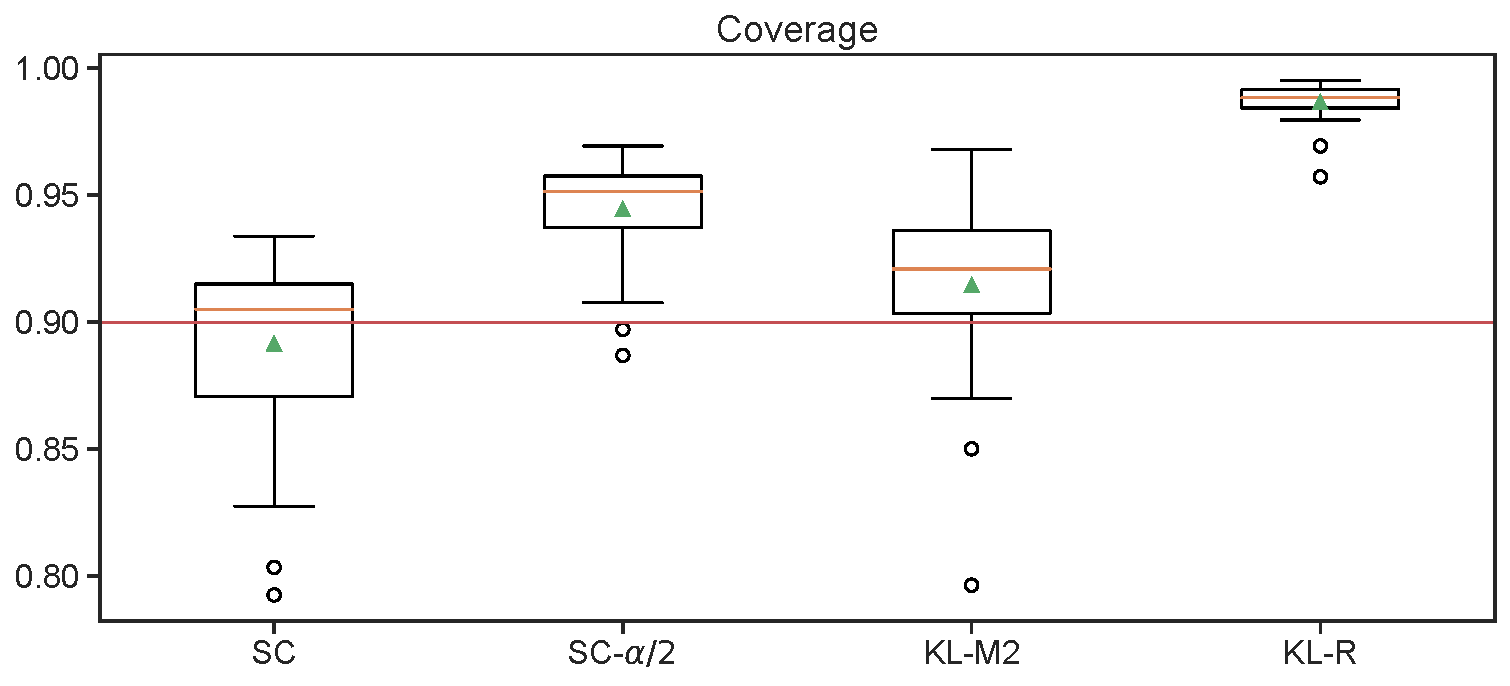
\includegraphics[width=0.9\linewidth]{covid/covid_rob_pred_ints_boxplot_Coverage_2021-10-05.pdf}
  \caption{Empirical coverage for the prediction sets generated by the standard conformal methodology (``SC''), the standard conformal methodology where we simply set $\alpha/2$ (``SC-$\alpha/2$''), and the Kullback-Leibler divergence on the COVID-19 time series.  We set $\rho$ according to the regression-based strategy (``KL-R'') for estimating the amount of shift that we describe in Section~\ref{sec:coverage-high-probability-over-shifts}, as well as via the nonparametric divergence estimator due to \citet{NguyenWaJo10} (``KL-M2'').  The horizontal red line marks the marginal coverage $.9$.}
  \label{fig:covid-coverage}
\end{figure}

\begin{figure}[ht]
  \centering
  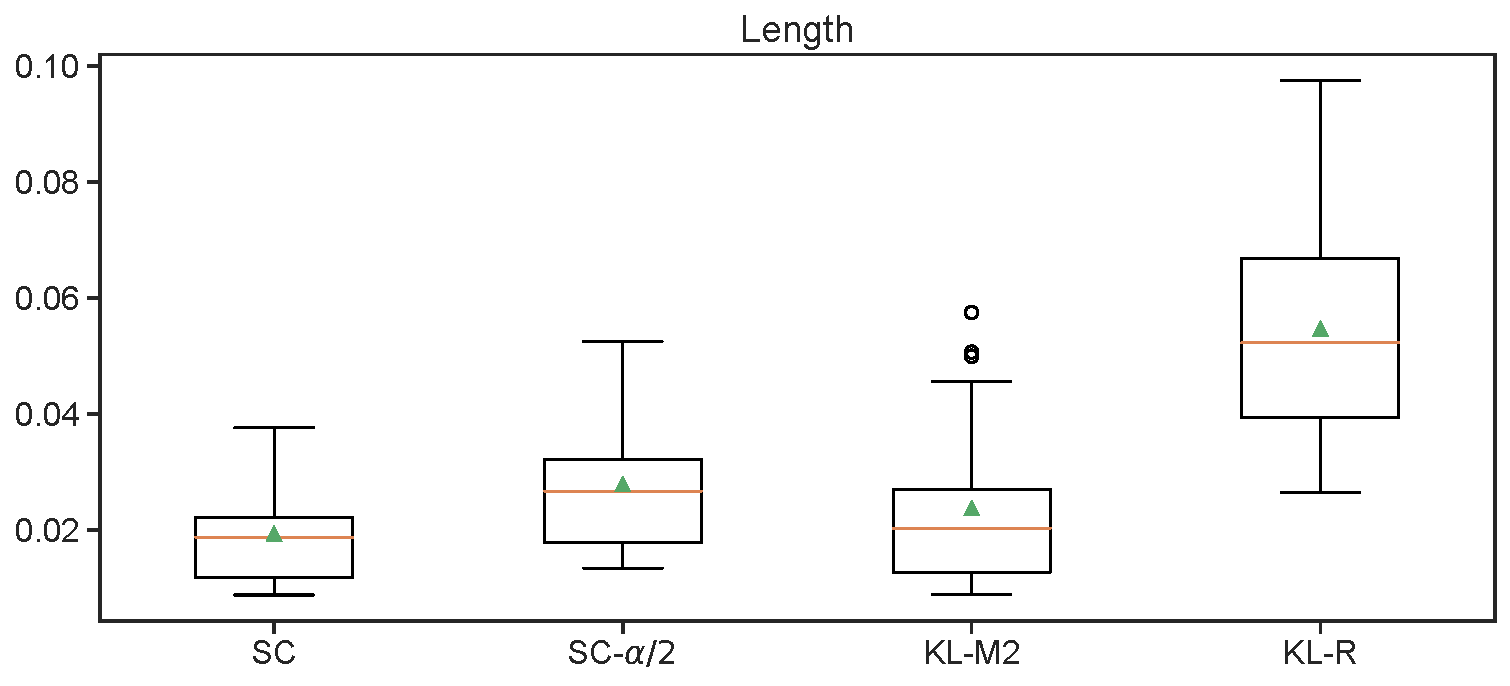
\includegraphics[width=0.9\linewidth]{covid/covid_rob_pred_ints_boxplot_Length_2021-10-05.pdf}
  \caption{Average length for the prediction intervals generated by the standard conformal methodology (``SC''), the standard conformal methodology where we simply set $\alpha/2$ (``SC-$\alpha/2$''), and the Kullback-Leibler divergence on the COVID-19 time series.  We set $\rho$ according to the regression-based strategy (``KL-R'') for estimating the amount of shift, as well as via the nonparametric divergence estimator due to \citet{NguyenWaJo10} (``KL-M2'').}
  \label{fig:covid-size}
\end{figure}

We view these results from a more qualitative perspective in Figures \ref{fig:covid-true} and \ref{fig:covid-hi-lo}.  In Figure \ref{fig:covid-true}, we show the actual number of COVID-19 cases on April 16, 2021, when the state of Michigan saw a sudden spike in the incidence of COVID-19 after several weeks of implementing precautionary measures.  As an especially pronounced example of distributional shift, it is natural to ask whether our procedures might offer any kind of protection in this instance.  Figure \ref{fig:covid-hi-lo} shows the upper and lower endpoints of the confidence intervals that our robust conformalization procedure generates at this point in time.  By comparing the colors in the figures, we can see that our robust prediction intervals generally contain the true response value both across the United States as well as in Michigan, in particular---despite the presence of such a severe distributional shift.

\begin{figure}[ht!]
  \centering
  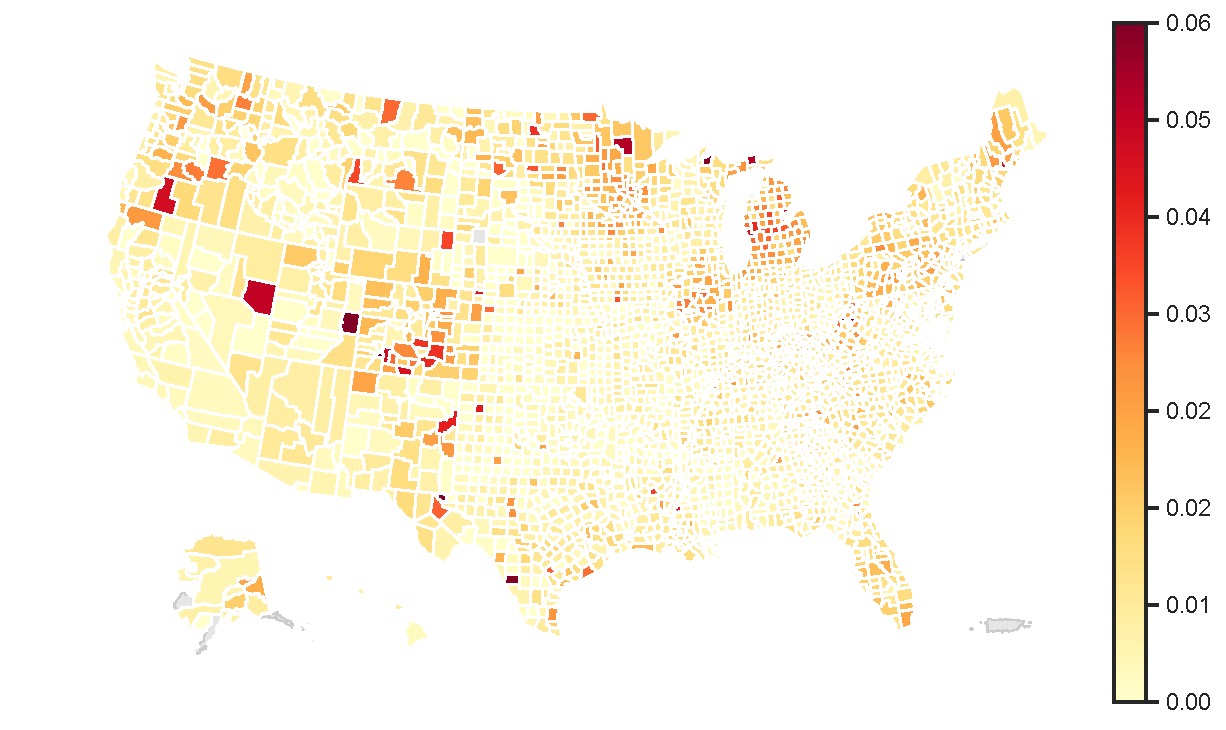
\includegraphics[width=0.9\linewidth]{covid/covid_rob_pred_ints_04-15-2021_true_alg_idx_0_cbar.pdf}
  \caption{The true (normalized) number of COVID-19 cases per 100{,}000 people, smoothed over the previous week, across the United States on April 16, 2021.}
  \label{fig:covid-true}
\end{figure}

\clearpage
\begin{figure}[h!]
  \centering
  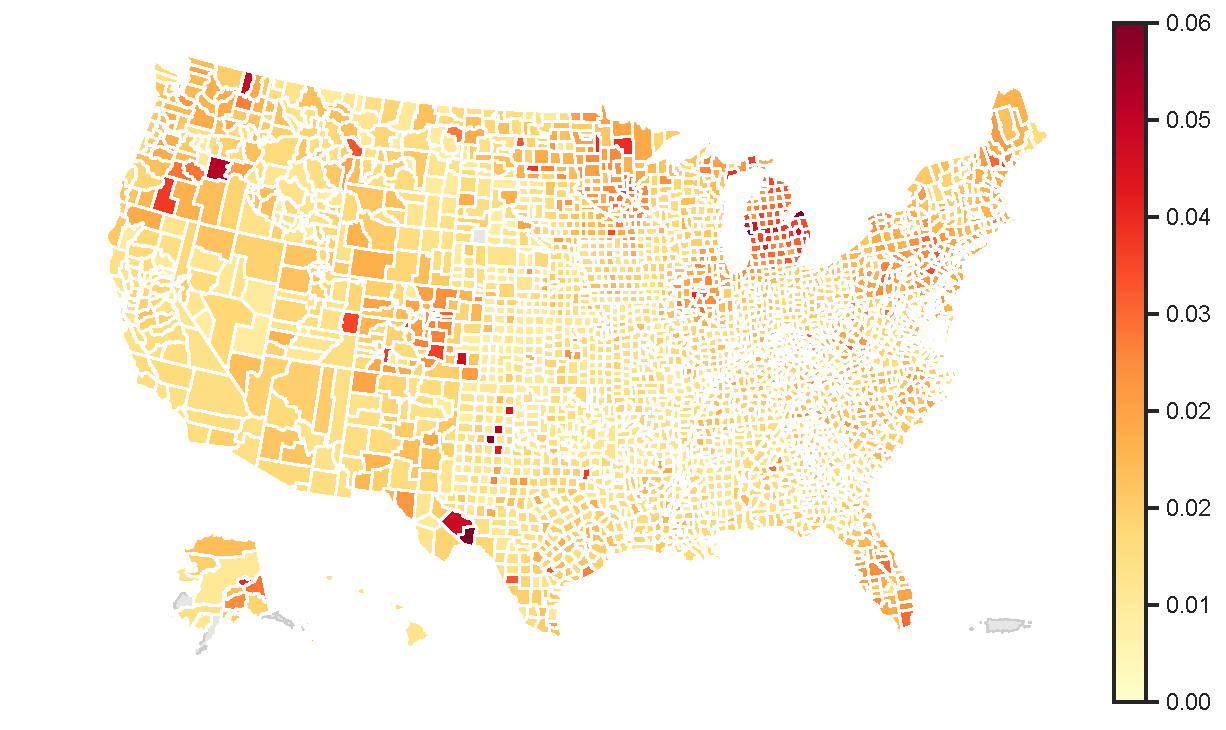
\includegraphics[width=0.9\linewidth]{covid/covid_rob_pred_ints_04-15-2021_his_alg_idx_0_cbar.pdf} \\
  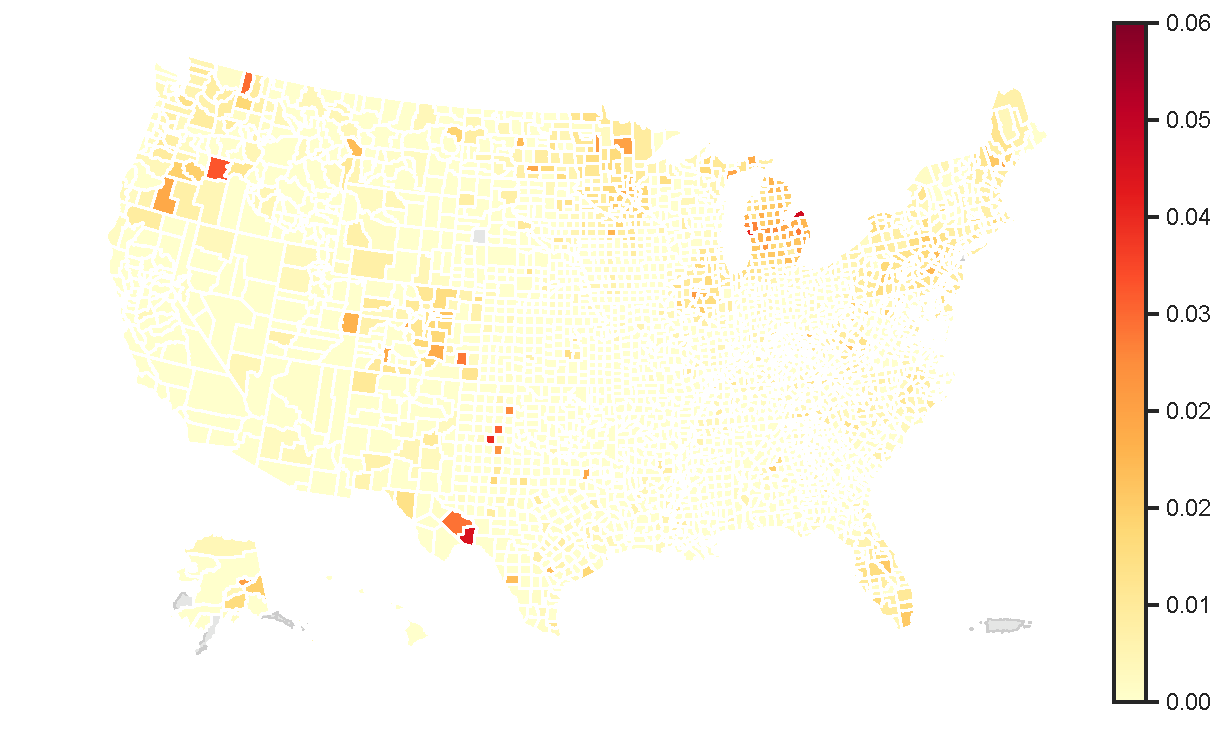
\includegraphics[width=0.9\linewidth]{covid/covid_rob_pred_ints_04-15-2021_los_alg_idx_0_cbar.pdf}
  \caption{The upper (top panel) and lower (bottom panel) endpoints of the confidence intervals that our robust conformal methodology generates across the United States on April 16, 2021.}
  \label{fig:covid-hi-lo}
\end{figure}
\clearpage

\subsection{Experiments on covariate sensitivity}
\label{sec:covariate-sensitivity}

Our final experiment is to evaluate our sensitivity predictions for
covariate shift, as in Sec.~\ref{sec:sensitivity}. The point is twofold: we
(i) identify covariates for which covarage may be sensitive, then (ii) test
whether these putative sensitivities are indeed present in data. To do so,
we consider three datasets from the UCI repository \citep{DuaGr17}:
real-estate data, weather history data, and wine quality data.

We repeat the following experiment 25 times:
we randomly partition each
dataset into disjoint sets $D_\train, D_\val, D_{\text{sens}}, D_\test$ each
containing respectively $40\%, 10\%,30\%,10\%$ of the data, then fit a
linear regression model $\mu$ using $D_\train$ and construct conformal
intervals of the form~\eqref{eqn:confidence-set} with $\score(x, y) =
|\mu(x)- y|$, so that $\what{C}_n(x) = \{y \in \R \mid |\mu(x) - y| \le
\hat{t}\}$, setting the threshold $\hat{t}$ so that we achieve coverage at
nominal level $\alpha = .1$ on $D_\val$.  We estimate the sensitivity
function using $D_{\text{sens}}$ as in Algorithm~\ref{alg:sensitivity1}
for each singleton covariate (i.e.\ the covariate set $I = \{i\}$ for
each of $i = 1, 2, \ldots$),
where we estimate the conditional probabilities of miscoverage using default
tuning parameeters in R's version of random forests.

Figure~\ref{fig:sens-fig} shows the results. The plot is somewhat complex:
for each of the three datasets, we estimate sensitivity (as a function of
shift $\rho$) for each covariate in the dataset (e.g.\ \texttt{House age} in
the real estate data). Then for an individual covariate, we plot (estimated)
maximum miscoverage as a function of the radius $\rho$ of potential shift in
that covariate (the estimated sensitivity function~\eqref{eqn:covsens-fcn},
where $I = \{i\}$ is the covariate of interest); this is the red solid line
in each plot. As we are curious about coverage losses under covariate
shifts, we plot miscoverage (dashed lines) on the subset of the test data
$D_\test$ containing examples either from the upper or lower $e^{-\rho}$
quantiles of each covariate, which corresponds to R\'{e}nyi
$\infty$-divergence $\rho$, as in Lemma~\ref{lemma:cvar-calc}.  We expect
that these miscoverages to fall below the maximum miscoverage line,
which we observe across all three datasets.
Specifically, we see that for real estate data, coverage of the
corresponding confidence sets drops most when the marginal distribution of
the covariate ``House age'' shifts while that for weather history data, the
coverage drops most for shifts in the ``Pressure'' covariate.  For the wine
quality dataset, coverage seems almost equally sensitive to all covariates.
An interesting question for future work is to identify those directions
which \emph{are} sensitive---as opposed to the approach here, which
identifies potentially sensitive covariates.

\begin{figure}
  \centering
\begin{overpic}[
  			   %grid, %		
  				scale=0.28]{%
     sensitivity/real-estate.pdf}
  \put(40, -1){
        \small Real estate data}
 \put(-1,10){
      \tikz{\path[draw=white, fill=white] (0, 0) rectangle (.3cm, 6cm)}
    }
   \put(-1,25){\rotatebox{90}{
      $\rho$}
    }
  \end{overpic}

%  \vspace{0.5in}
    \centering
  \begin{overpic}[
  			   %grid, %		
  				scale=0.28]{%
     sensitivity/weather-history.pdf}
  \put(40, -1){
        \small Weather history data }
 \put(-1,10){
      \tikz{\path[draw=white, fill=white] (0, 0) rectangle (.3cm, 6cm)}
    }
   \put(-1,20){\rotatebox{90}{
      $\rho$}
    }
  \end{overpic}

%  \vspace{0.5in}
    \centering
    \begin{overpic}[
  			   %grid, %		
  				scale=0.28]{%
     sensitivity/wine-quality.pdf}
  \put(40, -1){
        \small Wine quality data }
 \put(-1,10){
      \tikz{\path[draw=white, fill=white] (0, 0) rectangle (.3cm, 6cm)}
    }
   \put(-1,20){\rotatebox{90}{
      $\rho$}
    }
  \end{overpic}

  \vspace{0.2in}
 
  \caption{Sensitivity of (mis)-coverage for three datasets. Red line shows maximum miscoverage possible within a given shift in marginal distribution of a covariate with respect to limiting $f$-divergences. Dashed lines show miscoverage on a subset of test data that contains samples for which the corresponding covariate takes values in the upper or lower $e^{-\rho}$ quantiles of that covariate.}
  \label{fig:sens-fig}
\end{figure}
